\normaltrue
\correctiontrue

%\UPSTIidClasse{11} % 11 sup, 12 spé
%\newcommand{\UPSTIidClasse}{11}


\exer{Mouvement TT -- $\star$ \label{C2:09:03}}
\setcounter{question}{0}\UPSTIcompetence[2]{C2-09}
\index{Compétence C2-09}
\index{Principe fondamental de la dynamique}
\index{PFD}
\index{Mécanisme à 2 translations}
\ifcorrection
\else
\marginnote{\textbf{Pas de corrigé pour cet exercice.}}
\fi

\ifprof
\else
Soit le mécanisme suivant. On note $\vect{AB}=\lambda(t)\vect{i_0}$ et $\vect{BC}=\mu(t)\vect{j_0}$.
$G_1 = B$ désigne le centre d'inertie de \textbf{1},et $m_1$ sa masse et $\inertie{G_1}{1}=\matinertie{A_1}{B_1}{C_1}{0}{0}{0}{\bas{1}}$; 
$G_2 = C$ désigne le centre d'inertie de \textbf{2} et  $m_2$ sa masse  et $\inertie{G_2}{2}=\matinertie{A_2}{B_2}{C_2}{0}{0}{0}{\bas{2}}$.

 Un vérin électrique positionné entre \textbf{0} et \textbf{1} permet d'actionner le solide \textbf{1}.
 Un vérin électrique positionné entre \textbf{1} et \textbf{2} permet d'actionner le solide \textbf{2}.

L'accélération de la pesanteur est donnée par $\vect{g}=-g\vect{j_0}$.

\begin{center}
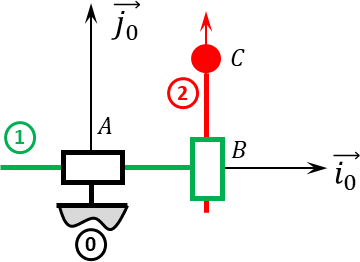
\includegraphics[width=.6\linewidth]{03_TT_01}
\end{center}
\fi

\question{Dans le but d'obtenir les lois de mouvement, appliquer le théorème de la résultante dynamique au solide \textbf{2} en projection sur $\vect{j_0}$.}
\ifprof

On isole \textbf{2}. 

\vspace{.25cm}

Bilan des actions mécaniques : 
\begin{itemize}
\item liaison glissière entre 1 et 2 : 
$\torseurstat{T}{1}{2}= \torseurl{X_{12}\vi{0}+Z_{12}\vk{0}}{L_{12}\vi{0}+M_{12}\vj{0}+N_{12}\vk{0}}{B}$;
\item pesanteur : $\torseurstat{T}{\text{Pes}}{2}= \torseurl{-m_2 g \vj{0}}{\vect{0}}{C}$;
\item vérin : $\torseurstat{T}{1_v}{2}= \torseurl{F_2 \vj{0}}{\vect{0}}{B}$.
\end{itemize}

\vspace{.25cm}

Application du TRD au solide \textbf{2} en projection sur $\vj{0}$: 

$\vectf{1}{2}\cdot \vj{0} + \vectf{\text{Pes}}{2}\cdot \vj{0}+ \vectf{1_v}{2}\cdot \vj{0} = \vectrd{2}{0}\cdot \vj{0}$.

\vspace{.25cm}

Calcul de la résultante dynamique : 
$\vectrd{2}{0} = m_2 \vectg{C}{2}{0} = m_2 \left(\lambdapp (t) \vi{0}+\mupp (t) \vj{0}\right)$.

Application du théorème : 
$$
-m_2g  + F_2 = m_2\mupp (t).
$$
\else
\fi


\question{Dans le but d'obtenir les lois de mouvement, appliquer le théorème de la résultante dynamique à l'ensemble \textbf{1+2} en projection sur $\vect{i_0}$}
\ifprof
On isole \textbf{1+2}. 

\vspace{.25cm}

Bilan des actions mécaniques : 
\begin{itemize}
\item liaison glissière entre 0 et 1 : 
$\torseurstat{T}{0}{1}= \torseurl{Y_{01}\vj{0}+Z_{12}\vk{0}}{L_{12}\vi{0}+M_{12}\vj{0}+N_{12}\vk{0}}{A}$;
\item pesanteur : $\torseurstat{T}{\text{Pes}}{1}= \torseurl{-m_1 g \vj{0}}{\vect{0}}{B}$;
\item pesanteur : $\torseurstat{T}{\text{Pes}}{2}= \torseurl{-m_2 g \vj{0}}{\vect{0}}{C}$;
\item vérin : $\torseurstat{T}{0_v}{1}= \torseurl{F_1 \vi{0}}{\vect{0}}{B}$.
\end{itemize}

\vspace{.25cm}

Application du TRD au solide \textbf{1+2} en projection sur $\vi{0}$: 

$\vectf{0}{1}\cdot \vi{0} + \vectf{\text{Pes}}{1}\cdot \vi{0}+ \vectf{\text{Pes}}{2}\cdot \vj{0}+ \vectf{0_v}{2}\cdot \vi{0} = \vectrd{1+2}{0}\cdot \vi{0}$.

\vspace{.25cm}

Calcul de la résultante dynamique : 
$\vectrd{1+2}{0} = m_1 \vectg{B}{1}{0}+m_2 \vectg{C}{2}{0} = m_1 \lambdapp (t) \vi{0} + m_2 \left(\lambdapp (t) \vi{0}+\mupp (t) \vj{0}\right)$.

Application du théorème : 
$$
F_1  + F_2 = m_1 \lambdapp (t)  + m_2 \lambdapp (t) .
$$

\else
\fi


\ifprof
\else
\begin{flushright}
\footnotesize{Corrigé  voir \ref{C2:09:03}.}
\end{flushright}%
\fi